\documentclass[a4paper]{article}
\usepackage[utf8]{inputenc}
\usepackage[italian]{babel}
\usepackage{import}
\usepackage{graphicx}
\usepackage{float}
\usepackage[margin=1.2in]{geometry}
\usepackage[12pt]{extsizes}
\usepackage{color}
\usepackage{listings}
\usepackage[bottom,flushmargin,hang,multiple]{footmisc}
\usepackage{titlesec}
\usepackage{url}
\usepackage{upquote}
\usepackage{biblatex}
\definecolor{purple}{RGB}{91, 72, 181}
\definecolor{darkviolet}{rgb}{0.58, 0.0, 0.83}
\definecolor{royalblue}{RGB}{242, 73, 214}
\definecolor{orange}{RGB}{227, 72, 41}
\definecolor{lightgreen}{RGB}{164, 194, 14}

\definecolor{mediumgray}{rgb}{0.3, 0.4, 0.4}
\definecolor{forestgreen}{rgb}{0.13, 0.55, 0.13}
\definecolor{crimson}{rgb}{0.86, 0.8, 0.24}

\addbibresource{./bibliografia/bibliografia.bib}

\linespread{1.5}

\graphicspath{ {./images/} }

\setcounter{secnumdepth}{4}
\setcounter{tocdepth}{4}

\titleformat{\paragraph}{\normalfont\normalsize\bfseries}{\theparagraph}{1em}{}
\titlespacing*{\paragraph}{0pt}{3.25ex plus 1ex minus .2ex}{1.5ex plus .2ex}

\lstset{aboveskip=30pt,belowskip=30pt}

\lstdefinestyle{JSES6Base}{
  backgroundcolor=\color{white},
  basicstyle=\ttfamily,
  breakatwhitespace=false,
  breaklines=false,
  captionpos=b,
  columns=fullflexible,
  commentstyle=\color{mediumgray}\upshape,
  emph={},
  emphstyle=\color{crimson},
  extendedchars=true,  % requires inputenc
  fontadjust=true,
  frame=single,
  identifierstyle=\color{black},
  keepspaces=true,
  keywordstyle=\color{purple},
  keywordstyle={[2]\color{darkviolet}},
  keywordstyle={[3]\color{royalblue}},
  keywordstyle={[4]\color{orange}},
  keywordstyle={[5]\color{lightgreen}},
  numbers=left,
  numbersep=5pt,
  numberstyle=\tiny\color{black},
  rulecolor=\color{black},
  showlines=true,
  showspaces=false,
  showstringspaces=false,
  showtabs=false,
  stringstyle=\color{forestgreen},
  tabsize=2,
  title=\lstname,
  upquote=true  % requires textcomp
}

\lstdefinestyle{JavaScript}{
  language=JavaScript,
  style=JSES6Base
}

\lstdefinestyle{ES6}{
  language=ES6,
  style=JSES6Base
}

\lstdefinelanguage{JavaScript}{
  morekeywords=[1]{break, continue, delete, else, for, function, if, in,
    new, return, this, typeof, var, void, while, with, render, getElementById, width, height},
  % Literals, primitive types, and reference types.
  morekeywords=[2]{false, null, true, boolean, number, undefined,
    Array, Boolean, Date, Math, Number, String, Object, onClick},
  morekeywords=[3]{h1, div, p, button, TextField},
  morekeywords=[4]{React, ., Component, Saluto, Convenevoli, Contatore, setContatore, useState, contatore,
    Button, ContatoreConTitolo},
  morekeywords=[5]{},
  sensitive,
  morecomment=[s]{/*}{*/},
  morecomment=[l]//,
  morecomment=[s]{/**}{*/}, % JavaDoc style comments
  morestring=[b]',
  morestring=[b]"
}[keywords, comments, strings]

\lstalias[]{ES6}[ECMAScript2015]{JavaScript}

\lstdefinelanguage[ECMAScript2015]{JavaScript}[]{JavaScript}{
  morekeywords=[1]{await, async, case, catch, class, const, default, do,
    enum, export, extends, finally, from, implements, import, instanceof,
    let, static, super, switch, throw, try},
  morestring=[b]` % Interpolation strings.
}


\title{Progettazione e realizzazione di un exchange decentralizzato per lo scambio di token ERC20 per la piattaforma CommonsHood}

\begin{document}
    \tableofcontents
    \newpage
    \section{Prerequisiti}
    \subsection{Blockchain}
    Una blockchain è un registro aperto e distribuito di dati, strutturato come una catena di blocchi contenenti le transazioni.
    I dati risiedono su unità computazionali chiamati \emph{nodi}, questi, come mostrato nell'immagine \ref{fig:node},
    sono interconnessi e comunicano tra loro per mantenere i dati di tutti i nodi aggiornati.\cite{nodo}
    \begin{figure}[h]
      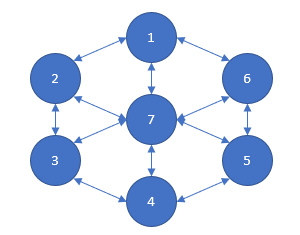
\includegraphics[scale=0.8]{node.png}
      \centering
      \caption{Rete di nodi}
      \centering
      \label{fig:node}
    \end{figure}
    \subsubsection{I nodi}
    Le responsabilità di un nodo sono principalmente:
    \begin{itemize}
      \item Controllo della validità di un nuovo record di dati, chiamato anche transazione, e acctettarlo o rifiutarlo;
      \item Nel caso di un record valido, salvataggio della transazione nel registro locale del nodo;
      \item Comunicazione e distribuzione della transazione agli altri nodi. In questo modo tutti i nodi hanno la stessa versione del registro.
    \end{itemize}
    \subsubsection{Le caratteristiche di una blockchain}
    Le caratteristiche principali della tecnologia blockchain sono:
    \begin{itemize}
      \item Decentralizzazione: le informazioni contenute nel registro digitale vengono distribuite tra più nodi, così da garantire sicurezza e resilienza dei sistemi anche in caso di attacco ad uno dei nodi o in caso di perdita di un nodo.
      \item Tracciabilità: ogni elemento salvato nel registro è tracciabile in ogni sua parte e se ne può risalire all’esatta provenienza e alle eventuali modifiche apportate nel corso del tempo, con una precisione assoluta.
      \item Disintermediazione: i singoli nodi della blockchain certificano le informazioni distribuite, rendendo quindi del tutto inutile la presenza di enti centrali o di aziende per la certificazione dei dati.
      \item Trasparenza: il contenuto del registro è visibile a tutti ed è facilmente consultabile e verificabile da ogni nodo della rete ma anche tramite servizi che interrogano la blockchain senza apportare modifiche. Nessuno può nascondere o modificare dati senza che l'intera rete venga a saperlo.
      \item Solidità del registro: dopo aver aggiunto un'informazione al registro, essa non può essere modificata senza il consenso di tutta la rete.
      \item Programmabilità: le operazioni di transazione possono anche essere programmate nel tempo, così da poter attendere il verificarsi di determinate condizioni prima di procedere con l'inserimento o la modifica.\cite{blockchain1}
    \end{itemize}
    \subsubsection{Smart contracts}
    Le blockchain permettono di implementare codici e funzioni all'interno di esse, questi sono chiamati smart contracts e permettono l'esecuzione di operazioni quando predeterminate condizioni si avverano.
    Sono tipicamente usate per automatizzare l'esecuzione di un accordo, in questo modo tutti i partecipanti possono verificarne immediatamente i risultati, senza aver bisogno di un itermediario.
    Possono, inoltre, essere utilizzate per automatizzare workflow, innescando azioni successive al raggiungimento di certe condizioni.\cite{smartcontracts}

    \subsection{Ethereum}
    Ethereum è una piattaforma blockchain decentralizzata che stabilisce una rete peer-to-peer che esegue e verifica smart contracts in modo sicuro.
    I smart contracts permettono transazioni tra gli utenti senza la necessità di un autorità centrale.
    Le transazioni sono immutabili, verificabili, e distribuiti in modo sicuro sulla rete. Le transazioni sono inviate e ricevute da account Ethereum creati dagli utenti.
    Come costo per il processamento di una transazione sulla rete, l'utente deve spendere Ether, la criptovaluta nativa di Ethereum.\cite{ethereum}
    \subsubsection{Token Ethereum}
    Ethereum permette la creazione di token crittografici all'interno della sua rete. Questi token non sono altro che smart contracts scritti seguendo specificazioni stabilite
    dagli sviluppatori della rete. I token possono essere di tipi di differenti, a seconda delle specificazioni seguite. In Ethereum ci sono pricipalmente due tipi di token: token ERC-20 e NFT.
    \paragraph{Token ERC-20}
    I token ERC-20 sono il tipo di token più diffuso sulla rete Ethereum, sono lo standard per la definizione di token fungibili\cite{erc20}, ossia i singoli token sono indistinguibili ed itercambiabili tra loro.
    Un token ERC-20 implementa le specificazioni indicate nell'EIP-20 che richiede nello smart contract del token la presenza di diversi metodi. I più importanti metodi richiesti sono:
    \begin{itemize}
      \item \verb|balanceOf(address _owner)|: restituisce la quantità di token posseduto da \verb|_owner|;
      \item \verb|transfer(address _to, uint256 _value)|: trasferisce una quantità di token indicata da \verb|_value| all'indirizzo \verb|_to|;
      \item \verb|transferFrom(address _from, address _to, uint256 _value)|: trasferisce una quantità \verb|_value| di token dall'indirizzo \verb|_from| all'indirizzo \verb|_to|;
      \item \verb|approve(address _spender, uint256 _value)|: permette all'indirizzo \verb|_spender| di ritirare fino a \verb|_value| token dall'account.\cite{eip20}
    \end{itemize}
    \paragraph{NFT}
    I Non Fungible Tokens sono, appunto, token non fungibili, ossia ogni token è univoco e non intercambiabile con un altro. Sono utilizzati per replicare le proprietà tipiche
    di un oggetto fisico come la scarsità, l'unicità e la possibilità di dimostrare la proprietà del token.\cite{nft}
    Data la natura del token, l'uso più comune di questi token è la creazione di arte digitale.\cite{nftuse}
    \newline
    Gli NFT seguono lo standard dettato dall'EIP-721.
    
    \subsection{OpenZeppelin}
    OpenZeppelin è una libreria per lo sviluppo di smart contracts sicuri. Le principali funzionalità fornite da OpenZeppelin sono:
    \begin{itemize}
    \item Implementazione dei diversi standard dei token Ethereum;
    \item Gestione del controllo degli accessi agli smart contracts;
    \item Componenti Solidity riutilizzabili per creare smart contracts.
    \end{itemize}

    \subsection{Metamask}
    Metamask è un'estensione del web browser. Questo software permette di connettere il browser con
    applicazioni decentralizzate basate sulla piattaforma Ethereum. Metamask permette la gestione di
    wallet Ethereum, la ricezione e l'invio di criptomonete basate su Ethereum, e l'interazione con
    applicazioni decentralizzate. L'estensione, inoltre, fornisce le API Ethereum web3, in questo
    modo le applicazioni sono in grado di leggere dati sulla blockchain.

    \subsection{ReactJS}
    React è una libreria JavaScript open-source per lo sviluppo di interfacce utente.
    \subsubsection{Caratteristiche di ReactJS}
    \paragraph{Componenti}
    I Componenti permettono di suddividere la UI in parti indipendenti, riutilizzabili e di pensare ad ognuna di esse in modo isolato.
    Per definire un componente è necessario implementare una funzione JavaScript, ad esempio:

    \begin{lstlisting}[style=ES6, title={Esempio componente}]
        function Saluto(props) {
            return <h1>Ciao, {props.nome}</h1>;
        }\end{lstlisting}

    Questo componente accetta un oggetto parametro contenente dati sotto forma di una singola
    "props", il quale è un oggetto parametro avente dati al suo interno.
    Per renderizzare un componente bisogna utilizzare la funzione \verb|ReactDOM.render()|,
    passandole come parametri il componente da visualizzare e il riferimento al componente padre.
    Se si volesse, quindi, renderizzare il componente \verb|Saluto|, passando "\emph{Martina}" come parametro \verb|nome|, il codice potrebbe essere:
    
    \begin{lstlisting}[style=ES6, title={Esempio composizione di componenti}]
      ReactDOM.render(
        <Saluto nome="Martina"/>, 
        document.getElementById('root')
      );\end{lstlisting}
    
    I componenti, inoltre, possono essere composte da altri componenti. In questo caso,
    renderizzando il componente padre, verranno visulizzati anche i componenti figli. Ad esempio, 
    si potrebbe avere un componente \verb|Convenevoli| che contiene multipli componenti \verb|Saluto|:
    \begin{lstlisting}[style=ES6, title={Esempio renderizzazione componente}]
      function Convenevoli() {
        return (
          <div>
            <Saluto nome="Sara" />
            <Saluto nome="Cahal" />
            <Saluto nome="Edite" />
          </div>
        );
      }\end{lstlisting}

      \paragraph{Hook state}
      Un componente React di default è stateless. Usando la funzione \verb|useState()| si può
      aggiungere uno stato interno ad un componente, React preserverà questo stato tra le ri-renderizzazioni.
      \verb|useState| ritorna una coppia: il valore dello stato corrente ed una funzione che ci permette di aggiornarlo.
      La funzione ha un unico parametro ed è il suo stato iniziale. Ad esempio, se si volesse realizzare un contatore con un bottone che, alla sua pressione,
      aumenti il valore del contatore, si potrebbe scrivere il seguente codice:
      \begin{lstlisting}[style=ES6, title={Esempio contatore con stato interno}]
        function Contatore() {
          const [contatore, setContatore] = useState(0);
          return (
            <div>
              <p>Hai cliccato {contatore} volte</p>
              <button 
                onClick={() => setContatore(contatore + 1)}>
                Cliccami
              </button>
            </div>
          );
        }
      \end{lstlisting}

      \paragraph{Hook effect}
      Il costrutto \verb|useEffect()| permette l'esecuzione di funzioni ad ogni renderizzazione da parte di React.
      Questa funzione viene utilizzata per effettuare operazioni nei vari stati del ciclo di vita di un componente.
      \newline
      Nel seguente esempio il titolo del documento viene aggiornato all'aumentare del valore del contatore, infatti, 
      ad ogni aggiornamento del DOM da parte di React, viene chiamata la funzione passata a \verb|useEffect()|.
      \begin{lstlisting}[style=ES6, title={Esempio uso di useEffect()}]
        function ContatoreConTitolo() {
          const [contatore, setContatore] = useState(0);

          useEffect(() => {
            document.title = `Hai cliccato ${contatore} volte`;
          });

          return (
            <div>
              <p>Hai cliccato {contatore} volte</p>
              <button
                onClick={() => setContatore(contatore + 1)}>
                Cliccami
              </button>
            </div>
          );
        }\end{lstlisting}

        \subsection{Material-UI}
        Material-UI è una libreria per ReactJS per creare interfacce utente.
        La libreria contiene al suo interno numerosi componenti grafici,
        questi sono forniti di un tema di default, per modificare l'aspetto di
        un componente si può utilizzare la sua proprietà \verb|className|.
        \newline
        Nell'esempio seguente vengono modificati le dimensione di un componente \verb|<Button>|:
        \begin{lstlisting}[style=ES6, title={Esempio modifica aspetto di un componente}]
          .Button {
            width: "100px",
            height: "100px"
          }

          <Button className="Button">
        \end{lstlisting}

        \subsection{Truffle e Ganache}
        Truffle e Ganache sono entrambi strumenti contenuti all'interno della suite software Truffle.
        Ganache permette la creazione di una blockchain Ethereum che viene eseguita in locale, semplificando, così,
        il deploy ed il test degli smart contracts. Truffle è un software che facilita lo sviluppo di smart contracts,
        i principali comandi di truffle utilizzati sono stati:
        \begin{itemize}
          \item \verb|truffle compile|, per compilare gli smart contracts;
          \item \verb|truffle test|, per eseguire i file di test;
          \item \verb|truffle deploy|, per eseguire il deploy degli smart contracts.
        \end{itemize}
        \newpage
        \section{Scrittura e test dei smart contracts}
        \newpage
        \section{Implementazione dell'interfaccia grafica}
        L'interfaccia utente che implementa le funzionalità di scambio di token è stata divisa in due pagine.
        La prima è chiamata \emph{Create Sale} e, scegliendo i token da vendere e quelli da accettare, permette
        la creazione di una vendita. La seconda è chiamata \emph{Sales List} e permette di visualizzare una lista di vendite, sia quelle in corso
        che quelle terminate.
        \subsection{Create Sale}
        Il processo di creazione di una vendita è diviso in tre step.
        Nel primo step viene permessso all'utente di scegliere i token in suo possesso da mettere in vendita.
        Nel secondo step l'utente sceglie i token che accetta come pagamento per la vendita dei token scelti nel primo step.
        Nel terzo step viene mostrato all'utente un riassunto delle scelte fatte nei due step precedenti, in questo passo, inoltre, l'utente può
        impostare una data di scadenza della vendita. Per mostrare graficamente il progresso nei diversi step è presente, in cima alla pagina, un componente
        \verb|<stepper>|, questo indica all'utente gli step terminati e quelli ancora da completare. 
        \subsubsection{Step 1: scelta dei token da vendere}
        \begin{figure}[h]
          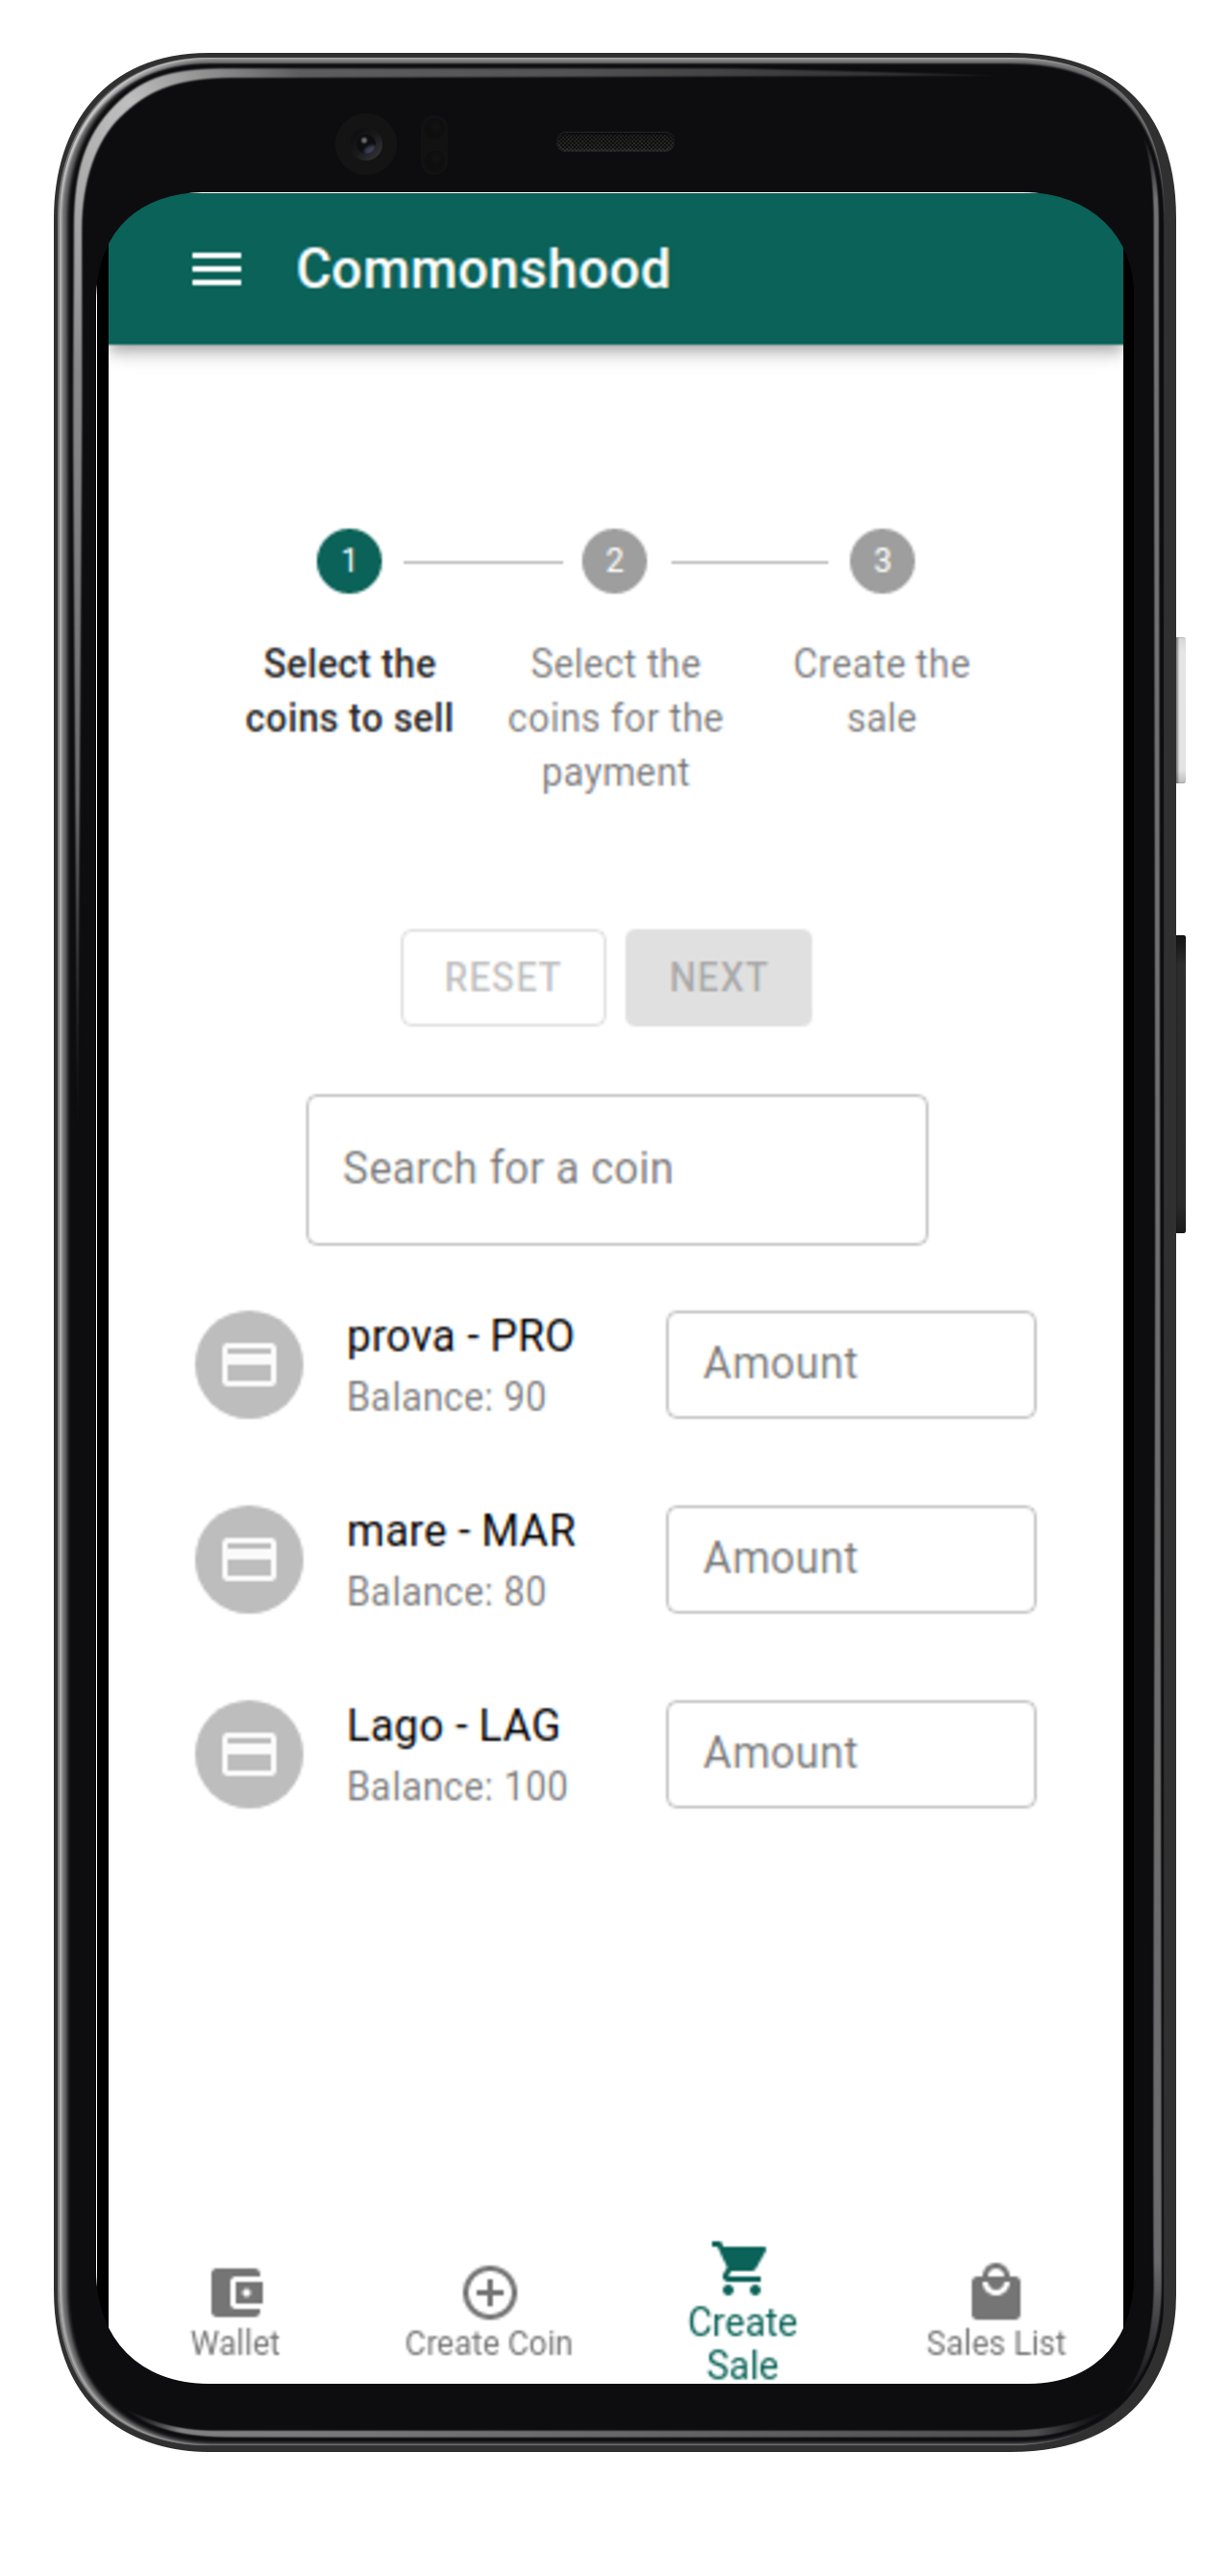
\includegraphics[width=\textwidth]{coinsToSell.png}
          \caption{Pagina per la scelta dei token in vendita}
          \centering
          \label{fig:resume}
        \end{figure}
        La pagina contiene una lista, creata usando il componente \verb|<List>|, ed una barra di ricerca, creata usando il componente \verb|<TextField>|.
        \newline
        Ogni elemento della lista contiene le informazioni di un token posseduto dall'utente e un componente
        \verb|<TextField>|, quest'ultimo permette l'inserimento della quantità desiderata del token da mettere in vendita.
        Gli eventi a cui la pagina reagisce possono essere divisi in tre categorie: caricamento della pagina, inserimento di quantità dei token e
        inserimento di testo nella barra di ricerca.
        \paragraph{Caricamento della pagina}
        Al caricamento della pagina vengono istanziate diverse variabili che gestiscono lo stato della stessa.
        \newpage
        \printbibliography
\end{document}